\documentclass[aps,prd,twocolumn,superscriptaddress,nofootinbib]{revtex4-2}

\usepackage{amsmath,amssymb}
\usepackage{graphicx}
\usepackage{hyperref}
\usepackage{xcolor}
\usepackage{booktabs}
\usepackage{tikz}
\usetikzlibrary{positioning,arrows.meta,calc}

% Custom commands
\newcommand{\epsg}{\ensuremath{\epsilon_{\text{gauge}}}}
\newcommand{\thetaP}{\ensuremath{\theta_P}}
\newcommand{\pyg}{\textsc{PyG}}
\newcommand{\todo}[1]{\textcolor{red}{[TODO: #1]}}

% Every number quoted inline is a generated macro (scripts/make_gauge_paper_tables.py)
% AUTO-GENERATED by scripts/make_gauge_paper_tables.py -- do not edit

% Macros are BARE MATH (no $..$): always use inside math mode.

\newcommand{\numAugMaxAbsR}{0.088}
\newcommand{\numBetaOneActionRA}{0.059 \pm 0.013}
\newcommand{\numBetaOneActionRB}{0.083 \pm 2 \times 10^{-4}}
\newcommand{\numCOracleActionRAtFifty}{0.87 \pm 0.06}
\newcommand{\numCOracleActionRAtFourHundred}{0.999 \pm 3 \times 10^{-4}}
\newcommand{\numCOracleWFourRFull}{0.476 \pm 0.011}
\newcommand{\numCOracleWFourRLSixteen}{0.316 \pm 0.009}
\newcommand{\numCollapseAugAFull}{1.1 \times 10^{-6}}
\newcommand{\numCollapseAugASmall}{1.4 \times 10^{-3}}
\newcommand{\numCollapseBaseAFull}{1.6 \times 10^{-6}}
\newcommand{\numCollapseBaseASmall}{2.5 \times 10^{-3}}
\newcommand{\numEpsABMax}{1.06}
\newcommand{\numEpsABMin}{0.95}
\newcommand{\numEpsBetaOneA}{0.990 \pm 0.033}
\newcommand{\numEpsBetaOneAWOne}{0.963 \pm 0.026}
\newcommand{\numEpsBetaOneB}{0.968 \pm 0.002}
\newcommand{\numEpsHatchMax}{1.06}
\newcommand{\numEpsHatchMin}{0.98}
\newcommand{\numEpsMatchABMax}{1.04}
\newcommand{\numEpsMatchABMin}{0.95}
\newcommand{\numHatchMaxAbsActionR}{0.041}
\newcommand{\numHatchMaxAbsAnyR}{0.094}
\newcommand{\numKCopies}{32}
\newcommand{\numMatchMaxAbsActionR}{0.062}
\newcommand{\numNumCCheckpointsExactZero}{36}
\newcommand{\numNumEpsCheckpoints}{148}
\newcommand{\numNumEpsRows}{50}


\begin{document}

\title{Learned versus Exact Gauge Invariance\\in Graph Neural Networks for Lattice Gauge Theory}

\author{Joshua Paul Brehm}
\email{joshua.paul.brehm@gmail.com}
\affiliation{Independent Researcher}

\date{\today}

\begin{abstract}
Neural-network surrogates for lattice gauge theory must respect gauge
symmetry, and the field has split between architectures that build the
symmetry in exactly and flexible architectures expected to learn it from
data. We test the learnable side of this divide directly in
two-dimensional compact U(1) lattice gauge theory. Three graph encodings
of the same gauge configurations---link variables as field nodes, link
variables as edge features, and a gauge-invariant plaquette oracle---are
trained under an identical protocol to regress the Wilson action, Wilson
loops, and the topological charge. The two link-level encodings fail
completely: predictions are uncorrelated with every gauge-invariant
target ($|r| \lesssim 0.1$), robustly across couplings, volumes,
parameter budgets, and training variations, while the oracle reaches
$r \approx 0.999$. A direct measurement of the gauge-invariance error
\epsg{}---the ratio of prediction variation along a gauge orbit to
variation across configurations---shows why: the link-level models sit
at $\epsg \approx 1$ everywhere, i.e.\ their outputs contain no
gauge-invariant component at all, whereas the oracle achieves
$\epsg = 0$ exactly. Retraining with random gauge transformations as
data augmentation does not move either number at any training-set size;
it merely shrinks the network output toward a constant, while the oracle
already reaches $r \approx 0.87$ from only 50 configurations. At this
model scale, gauge invariance is not learned at any price we could pay;
it must be supplied, through invariant inputs or equivariant
architecture.
\end{abstract}

\maketitle

%=============================================================================
\section{Introduction}
\label{sec:intro}
%=============================================================================

Machine-learned surrogates are increasingly used inside lattice field
theory workflows: as generative proposal distributions for exactness-preserving
samplers~\cite{Albergo2019,Kanwar2020,Boyda2021}, as part of a broader
program coupling lattice field theory to probabilistic machine
learning~\cite{Bachtis2021}, and as general-purpose emulators of local
theories~\cite{Favoni2022,Luo2021,Rayat2026,Brehm2026}. For gauge
theories, every such application confronts the same design decision.
Gauge symmetry is a \emph{redundancy}: physical observables are constant
on gauge orbits that occupy almost the entire configuration space. An
architecture can either enforce this exactly---through gauge-invariant
input features or gauge-equivariant network
operations~\cite{Kanwar2020,Boyda2021,Favoni2022,Luo2021,Rayat2026}---or
present raw link variables to a flexible model and rely on the data to
teach the symmetry.

The trade-off is usually argued qualitatively. Exact constructions
guarantee the symmetry but restrict the architecture to the group fixed
at design time; flexible architectures port across theories, boundary
conditions, and discretizations, but their symmetry error is rarely
measured. In a companion study of scalar $\phi^4$
theory~\cite{Brehm2026} we found the flexible side of this argument
convincing for \emph{spacetime} symmetries: a heterogeneous bipartite
graph neural network (GNN) with no built-in translation symmetry learned
it to high accuracy, transferred across lattice volumes, and matched
parameter-matched convolutional baselines. That paper deferred a sharper
question to this one: does the same flexibility-over-rigidity argument
survive contact with \emph{gauge} symmetry?

This paper answers that question quantitatively, and the answer is no.
Working in quenched two-dimensional compact U(1) lattice gauge
theory---small enough that every experiment is exactly validated and
cheaply repeatable---we train one GNN architecture on three graph
encodings of the same Monte Carlo ensembles
(Fig.~\ref{fig:variants}): link variables as first-class field nodes
(Variant~A), link variables as directed edge features (Variant~B), and
precomputed plaquette features, i.e.\ gauge-invariant inputs, as a
control (Variant~C). The targets are the Wilson action, Wilson loops of
five sizes, and the topological charge---all exactly gauge invariant.

Our contributions are threefold. First, a \emph{null result with
unusual robustness}: Variants A and B are statistically indistinguishable
from chance on every gauge-invariant target, across couplings, volumes,
seeds, matched parameter budgets, longer training, lower learning rates,
single-task objectives, and deeper message passing, while Variant~C is
at ceiling under the identical protocol (Sec.~\ref{sec:null}).
Second, a \emph{direct measurement of learned invariance}: we define a
per-target gauge-invariance error \epsg{} from the spread of predictions
over random gauge orbits and show that A and B sit at $\epsg \approx 1$
everywhere---their outputs are pure functions of the gauge
representative---while C achieves $\epsg = 0$ exactly, by a
bit-level argument about its inputs (Sec.~\ref{sec:eps}). Third, an
\emph{augmentation study}: retraining A and B with fresh random gauge
transformations of every training example, across training-set sizes
spanning two orders of magnitude, changes neither accuracy nor \epsg{};
the only effect is a collapse of the network output toward a constant
(Sec.~\ref{sec:aug}). The oracle, by contrast, reaches
$r=\numCOracleActionRAtFifty$ on the action from 50 configurations.

The interpretation is elementary but, we believe, worth establishing
experimentally: a single link variable is \emph{exactly} uninformative
about any gauge-invariant quantity, because a random gauge transformation
maps it to a uniformly distributed angle regardless of the underlying
physics (Sec.~\ref{sec:why}). Invariant information first appears in
oriented four-link products---plaquettes---so any learning signal is
invisible at first order in feature--target correlations, for the
supervised loss and for the augmentation-consistency loss alike. The
resulting optimization problem resembles learning a parity function:
possible in principle, but with no gradient to follow at realistic scale.
Gauge invariance, unlike translation invariance, is not an inductive
bias a flexible model acquires from data; it is a precondition for the
data to carry usable signal at all.

%=============================================================================
\section{Setup}
\label{sec:setup}
%=============================================================================

\textbf{Theory and ensembles.} We work with quenched compact U(1) gauge
theory on periodic $L \times L$ lattices, with link angles
$\theta_\mu(x) \in (-\pi,\pi]$, $U_\mu(x) = e^{i\theta_\mu(x)}$, and the
Wilson action~\cite{Wilson1974}
\begin{equation}
S[\theta] \;=\; \beta \sum_x \bigl[1 - \cos\thetaP(x)\bigr],
\label{eq:wilson}
\end{equation}
where the plaquette angle is
$\thetaP(x) = \theta_1(x) + \theta_2(x{+}\hat e_1) - \theta_1(x{+}\hat
e_2) - \theta_2(x)$. Ensembles of 4000 decorrelated configurations are
generated per $(\beta, L)$ point by a standard heatbath algorithm, for
$\beta \in \{0.5, 1, 2, 3, 4\}$ and $L \in \{8, 16, 32\}$, and validated
against the exact finite-volume mean plaquette of the 2D theory from the
character expansion
[$\langle \cos\thetaP \rangle \to I_1(\beta)/I_0(\beta)$ as
$V \to \infty$].

\textbf{Targets.} Each configuration is labeled with three families of
exactly gauge-invariant quantities: the total action
Eq.~\eqref{eq:wilson}; per-configuration Wilson loops $W(R,T)$, the
lattice average of $\cos$ of the oriented boundary angle sum of
$R \times T$ rectangles, for
$(R,T) \in \{(1,1),(2,2),(2,4),(3,3),(4,4)\}$; and the topological
charge $Q = \frac{1}{2\pi}\sum_x \widehat{\thetaP}(x)$, with
$\widehat{\thetaP}$ wrapped to $(-\pi,\pi]$, an exact integer on the
torus. Wilson-loop targets are the raw per-configuration values (not
$-\ln W$, which is undefined on the large fraction of configurations
with $W \le 0$ at large loop area). All targets are $z$-scored with
training-split statistics for loss balance; scale-dependent metrics are
computed after inverting the standardization, and Pearson $r$ is
unaffected by it.

\textbf{Model.} The architecture is the heterogeneous bipartite GNN of
Ref.~\cite{Brehm2026}, built on typed message
passing~\cite{Battaglia2018,Schlichtkrull2018,Hu2020} in
\pyg{}~\cite{FeyLenssen2019}: spacetime nodes carry a constant feature
(all geometry lives in displacement edge features, which restores exact
translation invariance), field content enters through dedicated node or
edge encoders, and $B$ residual message-passing blocks with layer
normalization propagate information before task heads read the result.
The action head sums a per-site MLP over spacetime nodes; Wilson-loop
and charge heads mean-pool all node types and apply an MLP, one head per
target. The coupling $\beta$ is appended to the input features and to
every head. Training follows the frozen protocol of
Ref.~\cite{Brehm2026}: AdamW, cosine schedule, 150 epochs, batch 32,
hidden width $H=64$, $B=3$ blocks, an 80/10/10
train/validation/test split, and 3--5 random seeds per cell.

%=============================================================================
\section{Three graph encodings of gauge links}
\label{sec:variants}
%=============================================================================

\begin{figure}[t]
\centering
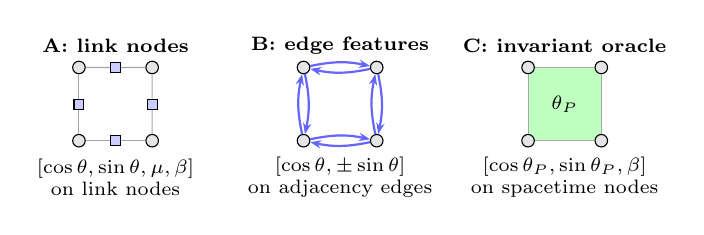
\begin{tikzpicture}[
  st/.style={circle, draw=black, fill=black!10, inner sep=1.6pt},
  ln/.style={rectangle, draw=black, fill=blue!20, inner sep=1.8pt},
  lk/.style={-, thick, blue!60},
  bi/.style={-, gray!70},
  scale=0.62, font=\scriptsize]
% ---------------- Variant A ----------------
\begin{scope}[xshift=0cm]
  \node at (0.75,1.95) {\textbf{A: link nodes}};
  \node[st] (a00) at (0,0) {};   \node[st] (a10) at (1.5,0) {};
  \node[st] (a01) at (0,1.5) {}; \node[st] (a11) at (1.5,1.5) {};
  \node[ln] (hb) at (0.75,0) {};   \node[ln] (ht) at (0.75,1.5) {};
  \node[ln] (vl) at (0,0.75) {};   \node[ln] (vr) at (1.5,0.75) {};
  \draw[bi] (a00) -- (hb); \draw[bi] (hb) -- (a10);
  \draw[bi] (a01) -- (ht); \draw[bi] (ht) -- (a11);
  \draw[bi] (a00) -- (vl); \draw[bi] (vl) -- (a01);
  \draw[bi] (a10) -- (vr); \draw[bi] (vr) -- (a11);
  \node[align=center] at (0.75,-0.75)
    {$[\cos\theta,\sin\theta,\mu,\beta]$\\on link nodes};
\end{scope}
% ---------------- Variant B ----------------
\begin{scope}[xshift=4.6cm]
  \node at (0.75,1.95) {\textbf{B: edge features}};
  \node[st] (b00) at (0,0) {};   \node[st] (b10) at (1.5,0) {};
  \node[st] (b01) at (0,1.5) {}; \node[st] (b11) at (1.5,1.5) {};
  \foreach \p/\q in {b00/b10, b01/b11, b00/b01, b10/b11} {
    \draw[lk,-{Stealth[length=4pt]}] (\p) to[bend left=12] (\q);
    \draw[lk,-{Stealth[length=4pt]}] (\q) to[bend left=12] (\p);
  }
  \node[align=center] at (0.75,-0.75)
    {$[\cos\theta,\pm\sin\theta]$\\on adjacency edges};
\end{scope}
% ---------------- Variant C ----------------
\begin{scope}[xshift=9.2cm]
  \node at (0.75,1.95) {\textbf{C: invariant oracle}};
  \fill[green!25] (0,0) rectangle (1.5,1.5);
  \node[st] (c00) at (0,0) {};   \node[st] (c10) at (1.5,0) {};
  \node[st] (c01) at (0,1.5) {}; \node[st] (c11) at (1.5,1.5) {};
  \draw[bi] (c00)--(c10)--(c11)--(c01)--(c00);
  \node at (0.75,0.75) {$\thetaP$};
  \node[align=center] at (0.75,-0.75)
    {$[\cos\thetaP,\sin\thetaP,\beta]$\\on spacetime nodes};
\end{scope}
\end{tikzpicture}
\caption{Three graph encodings of the same U(1) configuration
(one plaquette shown). \textbf{A}: each of the $2L^2$ links is a field
node attached to its two endpoint sites by typed edges; message passing
alternates link$\to$site, site$\to$site, site$\to$link. \textbf{B}:
links ride as features on the directed site--site adjacency edges, with
the reversed edge carrying the inverse link $[\cos\theta,-\sin\theta]$.
\textbf{C} (control): each site carries the trigonometric features of
its plaquette---inputs that are gauge invariant \emph{by construction}.
A plaquette is a 4-link neighborhood: in A and B its information becomes
available within two message-passing blocks.}
\label{fig:variants}
\end{figure}

The experiment hinges on presenting identical physics to identical
learning machinery under encodings that differ only in \emph{where the
gauge redundancy lives} (Fig.~\ref{fig:variants}).

\textbf{Variant A (link nodes)} is the natural extension of the
fields-as-nodes thesis of Ref.~\cite{Brehm2026}: every link is a field
node with features $[\cos\theta, \sin\theta,
\mathrm{onehot}(\mu), \beta]$, connected to its endpoint sites by typed
directed edges, with a three-stage message-passing block
(link$\to$site, site$\to$site, site$\to$link).

\textbf{Variant B (edge features)} attaches $[\cos\theta, \sin\theta]$
to the existing directed site--site adjacency edges, alongside the
displacement features; the reversed edge carries the inverse link
$[\cos\theta, -\sin\theta]$. Only spacetime nodes remain.

\textbf{Variant C (invariant oracle)} precomputes the one independent
plaquette per site in 2D and places $[\cos\thetaP, \sin\thetaP, \beta]$
on the spacetime nodes. This is the information-level ceiling: the model
is handed gauge invariance and asked only to compose invariants into
targets. It is a control, not a proposal---in higher dimensions or for
larger structures, enumerating all invariants is exactly the expense one
hopes a learned model avoids.

At fixed width $H=64$, Variant A carries $2.5\times$ the parameters of
B and C (296k vs.\ 118k), because of its extra encoder and per-block
message functions. We therefore run the comparison in both a fixed-$H$
arm and a parameter-matched arm (B, C widened to $H=102$ to match A's
budget; A narrowed to $H=40$ to match B's).

%=============================================================================
\section{Results}
\label{sec:results}
%=============================================================================

\subsection{Learned invariance does not happen}
\label{sec:null}

\begin{table*}[t]
\caption{A/B/C comparison on gauge-invariant targets (test split, mean
$\pm$ std over seeds; 3 seeds for A/B, 5 for C). $Q$ acc.\ is
exact-integer accuracy after rounding. Variants A and B are at chance on
every target, up to the percent-level $\beta=1$ correlation discussed in
the text; the invariant oracle C is at ceiling except for the
receptive-field-limited $4\times4$ loop (Sec.~\ref{sec:oracle}).}
\label{tab:abc}
\centering
% AUTO-GENERATED by scripts/make_gauge_paper_tables.py -- do not edit

\begin{tabular}{@{}clcrcccc@{}}
\toprule
Variant & $L$ & $\beta$ & Params & Action $r$ & $W_{1\times1}$ $r$ & $W_{4\times4}$ $r$ & $Q$ acc. \\
\midrule
A & 8 & 1 & 296k & $0.059 \pm 0.013$ & $0.080 \pm 0.005$ & $0.065 \pm 0.009$ & $0.255 \pm 0.000$ \\
A & 8 & 2 & 296k & $-0.017 \pm 0.027$ & $-0.004 \pm 0.016$ & $-0.015 \pm 0.033$ & $0.373 \pm 0.000$ \\
A & 16 & 2 & 296k & $0.036 \pm 0.105$ & $-0.012 \pm 0.028$ & $0.050 \pm 0.026$ & $0.145 \pm 0.000$ \\
\addlinespace
B & 8 & 1 & 118k & $0.083 \pm 2 \times 10^{-4}$ & $0.086 \pm 0.001$ & $0.040 \pm 0.008$ & $0.255 \pm 0.000$ \\
B & 8 & 2 & 118k & $-0.057 \pm 0.002$ & $-0.060 \pm 0.006$ & $-0.008 \pm 0.057$ & $0.373 \pm 0.000$ \\
B & 16 & 2 & 118k & $0.014 \pm 0.012$ & $0.046 \pm 0.012$ & $0.030 \pm 0.036$ & $0.145 \pm 0.000$ \\
\addlinespace
C & 8 & 1 & 118k & $1.000 \pm 6 \times 10^{-5}$ & $0.999 \pm 2 \times 10^{-4}$ & $0.021 \pm 0.026$ & $0.984 \pm 0.003$ \\
C & 8 & 2 & 118k & $0.999 \pm 3 \times 10^{-5}$ & $0.999 \pm 9 \times 10^{-5}$ & $0.476 \pm 0.011$ & $0.997 \pm 0.001$ \\
C & 16 & 2 & 118k & $0.999 \pm 7 \times 10^{-5}$ & $0.998 \pm 0.001$ & $0.316 \pm 0.009$ & $0.981 \pm 0.007$ \\
\bottomrule
\end{tabular}

\end{table*}

Table~\ref{tab:abc} shows the headline comparison at the three
$(\beta, L)$ cells where all variants were trained. Variants A and B are
statistically indistinguishable from chance on the action, all five
Wilson-loop sizes, and the topological charge; $Q$ ``accuracy'' equals
the base rate of the modal charge sector. Variant C, trained under the
identical protocol, reaches $r \ge 0.997$ on the action and short-distance
loops.

We stress-tested the null before accepting it. It persists at every
A/B cell trained ($\beta \in \{1,2\}$, $L \in \{8,16\}$, three seeds
each), while C's ceiling holds over its full matrix
($\beta \in \{0.5,\dots,4\}$ at $L \in \{8,16\}$; $\beta \in \{1,2,4\}$
at $L=32$); under both directions of parameter matching
(max $|r| = \numMatchMaxAbsActionR$ on the action); and under four
targeted escape hatches for Variant A---$3\times$ longer training, a
lower learning rate with $2\times$ training, a single-task objective on
the most local target $W(1{\times}1)$ alone, and a deeper $B=6$ stack
(max $|r| = \numHatchMaxAbsActionR$ on the action,
$\numHatchMaxAbsAnyR$ over all targets). Training loss decreases in
every case, but only to the constant-predictor floor: the networks
converge to predicting the per-target mean, not to fitting individual
training configurations, and no generalizing signal appears.

The single systematic exception is at $\beta = 1$, where both variants
show a small but seed-consistent action correlation
(A: $r = \numBetaOneActionRA$, B: $r = \numBetaOneActionRB$). We return
to it below; it is the exception that maps the boundary of the null.

\subsection{The gauge-invariance error}
\label{sec:eps}

Accuracy alone cannot distinguish ``failed to learn the physics'' from
``failed to learn the symmetry.'' We therefore measure invariance
directly. For each test configuration $\theta_i$ we draw $K=\numKCopies$
random gauge transformations
$\theta_\mu(x) \to \theta_\mu(x) + \alpha(x) - \alpha(x{+}\hat e_\mu)$
with i.i.d.\ $\alpha(x) \sim \mathrm{U}(-\pi,\pi]$, and define, per
prediction head $\hat y$,
\begin{equation}
\epsg \;=\;
\frac{\bigl\langle \operatorname{std}_{g}\,
      \hat y(g \cdot \theta_i) \bigr\rangle_i}
     {\operatorname{std}_i\, \hat y(\theta_i)},
\label{eq:eps}
\end{equation}
the mean prediction spread along gauge orbits in units of the prediction
spread across configurations. A gauge-invariant predictor has
$\epsg = 0$; a predictor that responds to the gauge representative as
strongly as to the physics has $\epsg \approx 1$. The ratio is invariant
under affine rescaling of $\hat y$, so it can be evaluated on the
model's standardized output scale.

Two protocol details matter. First, gauge copies are generated in
float64 from the float32-stored links; the resulting
$\sim\!10^{-15}$ transformation noise in $\cos\thetaP$, $\sin\thetaP$ is
seven orders of magnitude below float32 feature resolution, so Variant
C's \emph{inputs are bit-identical} across each orbit. Its $\epsg = 0$
rows in Table~\ref{tab:eps} are exact, a built-in sanity anchor for the
pipeline. Second, achieving that exactness requires evaluating each
graph unbatched: batched message passing is position-in-batch dependent
at float32 machine precision ($\sim\!10^{-8}$ output differences between
bit-identical graphs at different batch positions), which would
otherwise put a spurious floor under the oracle's zero.

\begin{table*}[t]
\caption{Gauge-invariance error \epsg{} [Eq.~\eqref{eq:eps}, $K=\numKCopies$
gauge copies per test configuration] by target: total action $S$, Wilson
loops, topological charge $Q$. Mean $\pm$ std over seeds. Variant C's
zeros are exact (bit-identical inputs; see text). Across all
\numNumEpsRows{} measured cells---including parameter-matched budgets,
escape hatches, and every augmentation arm---A and B lie in
$\epsg \in [\numEpsABMin, \numEpsABMax]$.}
\label{tab:eps}
\centering
% AUTO-GENERATED by scripts/make_gauge_paper_tables.py -- do not edit

\begin{tabular}{@{}clccccc@{}}
\toprule
Variant & $L$ & $\beta$ & $\epsg^{S}$ & $\epsg^{W_{1\times1}}$ & $\epsg^{W_{4\times4}}$ & $\epsg^{Q}$ \\
\midrule
A & 8 & 1 & $0.990 \pm 0.033$ & $0.963 \pm 0.026$ & $0.959 \pm 0.020$ & $0.973 \pm 0.019$ \\
A & 8 & 2 & $1.000 \pm 0.013$ & $0.989 \pm 0.009$ & $1.015 \pm 0.012$ & $0.996 \pm 0.003$ \\
A & 16 & 2 & $1.002 \pm 0.018$ & $1.008 \pm 0.009$ & $1.028 \pm 0.007$ & $1.011 \pm 0.005$ \\
\addlinespace
B & 8 & 1 & $0.968 \pm 0.002$ & $0.976 \pm 0.005$ & $0.967 \pm 0.009$ & $1.005 \pm 0.045$ \\
B & 8 & 2 & $1.012 \pm 0.005$ & $1.026 \pm 0.010$ & $1.020 \pm 0.022$ & $1.008 \pm 0.029$ \\
B & 16 & 2 & $1.005 \pm 0.031$ & $1.026 \pm 0.017$ & $1.047 \pm 0.028$ & $1.033 \pm 0.021$ \\
\addlinespace
C & 8 & 1 & $0$ & $0$ & $0$ & $0$ \\
C & 8 & 2 & $0$ & $0$ & $0$ & $0$ \\
C & 16 & 2 & $0$ & $0$ & $0$ & $0$ \\
\bottomrule
\end{tabular}

\end{table*}

Table~\ref{tab:eps} gives the result. Variants A and B sit at
$\epsg \approx 1$ on every head: their predictions vary as much when the
gauge is changed at fixed physics as when the physics itself changes.
The trained functions contain \emph{no gauge-invariant component}. This
is a strictly stronger statement than the accuracy null---these models
did not learn a noisy approximation to an invariant observable; they
learned nothing invariant at all. The same holds for the
parameter-matched arm ($\epsg \in [\numEpsMatchABMin,\numEpsMatchABMax]$)
and all four escape hatches
($\epsg \in [\numEpsHatchMin,\numEpsHatchMax]$), over
\numNumEpsCheckpoints{} checkpoints in total; every one of the
\numNumCCheckpointsExactZero{} Variant-C checkpoints returns exactly
zero.

The $\beta = 1$ exception is visible here too, from the other side:
both link-level variants dip a few percent below unity
(B: $\epsg = \numEpsBetaOneB$ on the action head;
A: $\numEpsBetaOneAWOne$ on the $W_{1\times1}$ head)---the size expected
from a percent-level invariant component,
consistent with the small $r$ observed at that coupling. We interpret
this as a weak-coupling foothold: at small $\beta$ the plaquette
distribution is broad, and low-order combinations of nearby links carry
slightly more usable signal relative to the gauge noise. The foothold
does not grow with data or training in any experiment we ran.

\subsection{Augmentation does not buy invariance}
\label{sec:aug}

\begin{figure*}[t]
\centering
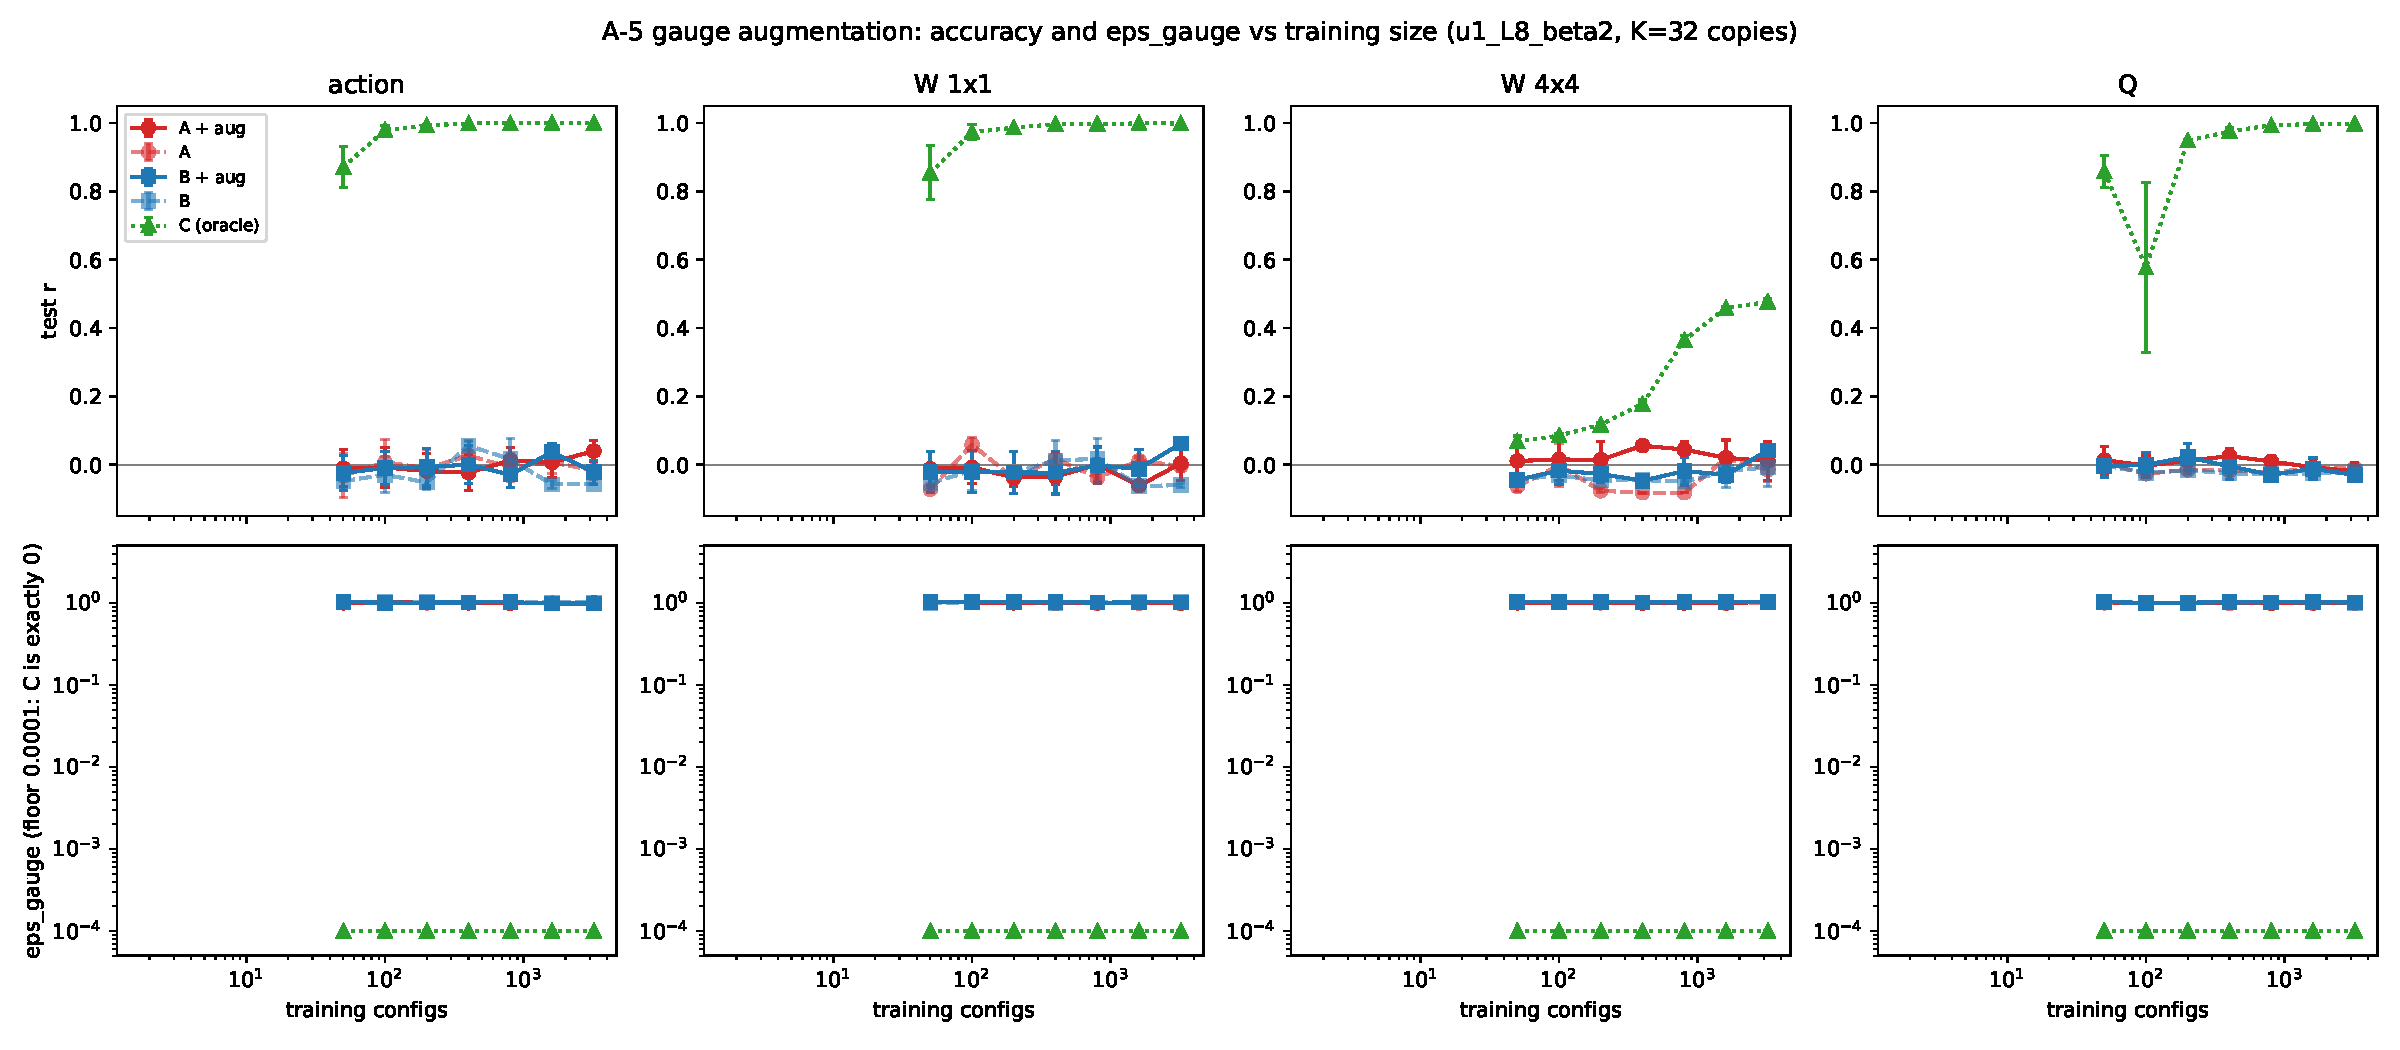
\includegraphics[width=\textwidth]{figures/a5_augmentation.pdf}
\caption{Gauge-transform data augmentation does not rescue the
link-level encodings ($L=8$, $\beta=2$; 3 seeds per point; the $C$
$n{=}3200$ reference uses the 5-seed protocol runs). \textbf{Top:} test
Pearson $r$ vs.\ training-set size for the action, two Wilson-loop
sizes, and the topological charge. Variants A and B, with (solid) and
without (dashed) on-the-fly random gauge augmentation, remain at chance
at every size ($|r| \le \numAugMaxAbsR$ across all arms, sizes, and
targets), while the invariant oracle C (green) reaches
$r = \numCOracleActionRAtFifty$ on the action from 50 configurations and
$\numCOracleActionRAtFourHundred$ by 400. \textbf{Bottom:} \epsg{} for
the same runs stays at unity for A and B at every size---augmentation
never produces an invariant component; C is exactly zero (plotted at the
$10^{-4}$ axis floor).}
\label{fig:aug}
\end{figure*}

If the missing ingredient were merely an invariance \emph{prior}, the
standard remedy would be data augmentation: draw a fresh random gauge
transformation of every training configuration at every access, so the
model sees each physical state under an ever-changing gauge and the loss
itself penalizes gauge dependence. The labels, being exactly invariant,
transfer unchanged; augmentation costs nothing but compute.

Figure~\ref{fig:aug} shows the outcome across training-set sizes
$n \in \{50, \dots, 3200\}$, with matched unaugmented baselines and the
oracle as reference. Augmentation changes nothing that matters. Test
correlations remain at chance for both variants at every $n$ (and in a
full-size check at $L=16$); \epsg{} remains at unity for every head at
every $n$. What augmentation \emph{does} do---visible only in the
components of Eq.~\eqref{eq:eps}---is drive the network toward the
trivial invariant: the constant function. The config-to-config spread of
the augmented Variant-A action head falls from $\numCollapseAugASmall$
(standardized units, $n=50$) to $\numCollapseAugAFull$ ($n=3200$); the
unaugmented arm follows the same trajectory
($\numCollapseBaseASmall$ to $\numCollapseBaseAFull$) as ordinary
training regresses an unlearnable target toward its mean. In both cases
the \emph{residual} fluctuation is pure gauge noise---which is why the
ratio \epsg{} stays pinned at unity while both of its ingredients
collapse by three orders of magnitude. Optimization can damp the
gauge-covariant component of the function; at this scale it never
rotates it into the invariant subspace.

The contrast with the oracle's data efficiency quantifies what exact
invariance is worth: Variant C reaches $r = \numCOracleActionRAtFifty$
on the action with 50 training configurations---fewer samples than the
model has layers of width 64---and is at ceiling by a few hundred. Handing
the model the invariant is worth more than any amount of augmented data
we could supply.

\subsection{What the oracle does with the same budget}
\label{sec:oracle}

\begin{figure}[t]
\centering
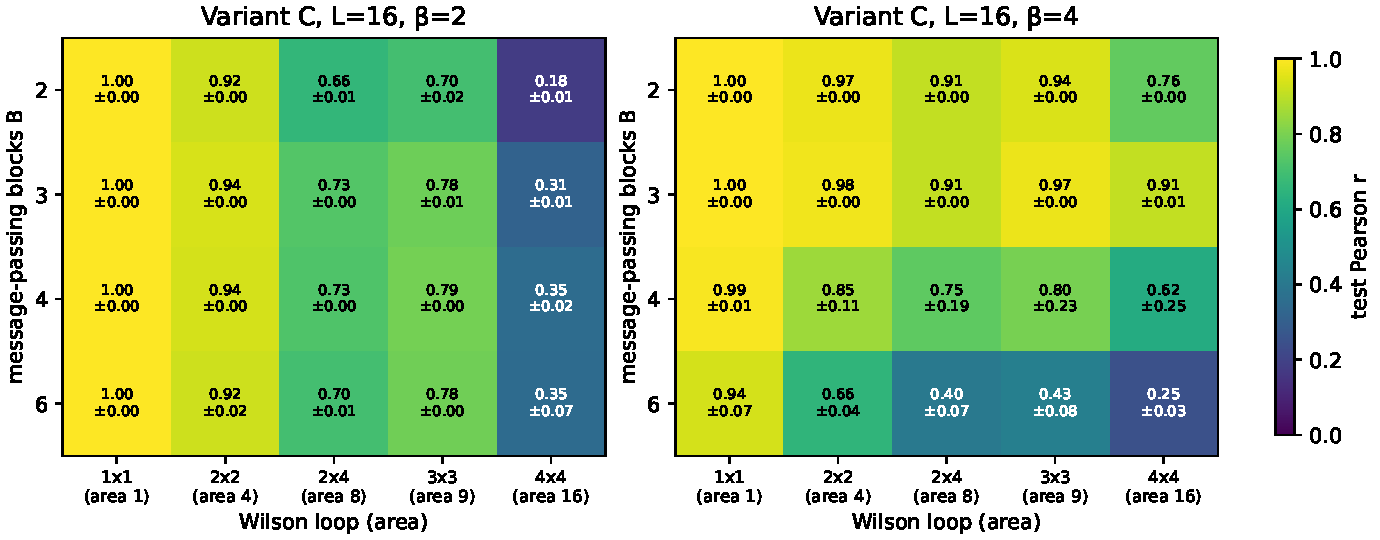
\includegraphics[width=\columnwidth]{figures/a4_receptive_field.pdf}
\caption{Receptive-field study on the invariant oracle (Variant C,
$L=16$): test $r$ for Wilson loops of increasing area vs.\ message-passing
depth $B$, at $\beta=2$ (disordered) and $\beta=4$ (ordered). Depth
extends the reachable loop size at $\beta=2$ but degrades large-loop
readouts at $\beta=4$ (the $Q$ readout of the same runs collapses to
base rate at $B=6$; see text).}
\label{fig:rf}
\end{figure}

\begin{figure}[t]
\centering
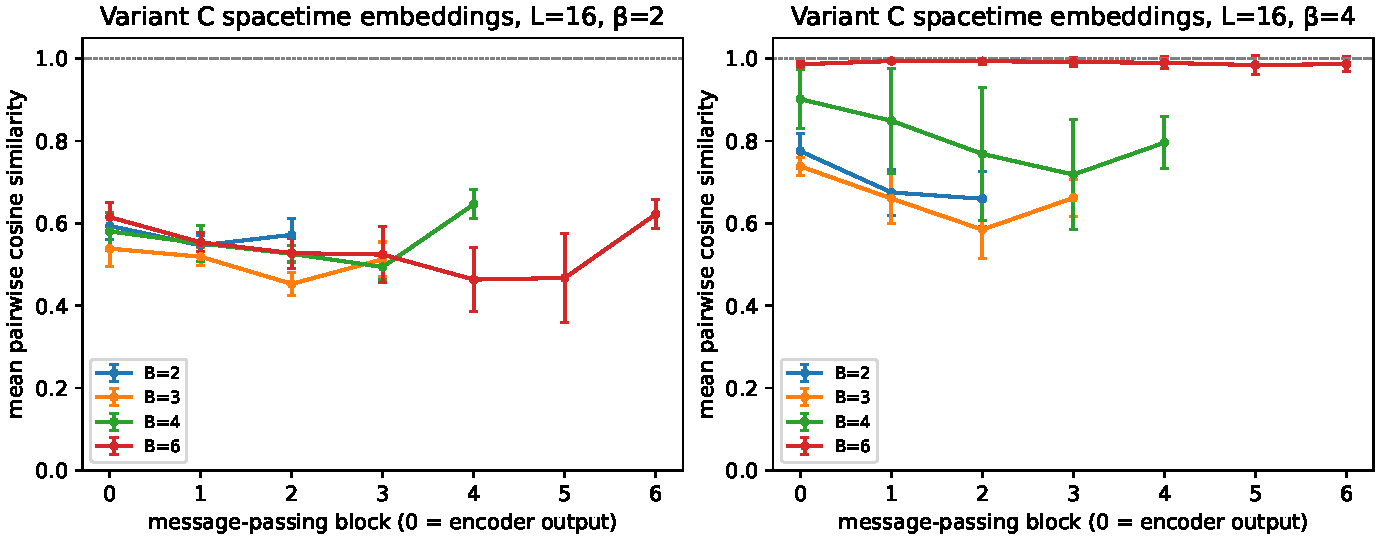
\includegraphics[width=\columnwidth]{figures/a4_oversmoothing.pdf}
\caption{Over-smoothing diagnostic on trained oracle models
($\beta=2$ and $\beta=4$ panels): mean pairwise cosine similarity of
spacetime-node embeddings after each message-passing block. Deep stacks
at $\beta=4$ collapse the node representations (two seeds reach
identical embeddings), while $\beta=2$ models stay healthy at every
depth; per-seed collapse predicts per-seed readout failure.}
\label{fig:oversmooth}
\end{figure}

Variant C's failures are as informative as its successes, because they
calibrate what even an invariant-input model cannot do at this scale.
Two systematic effects appear (Figs.~\ref{fig:rf}
and~\ref{fig:oversmooth}).

\emph{Receptive field.} Prediction quality for $W(R,T)$ falls with loop
area at fixed depth---$r = \numCOracleWFourRLSixteen$ for the $4\times4$
loop at $B=3$, $L=16$, $\beta=2$ with the full training set---and, in
the disordered phase, recovers with added depth, tracking the number of
lattice spacings a node can see. This turns the locality interpretation of
Ref.~\cite{Brehm2026} into a measured scaling and sets the depth budget
a Phase-scale application must plan for.

\emph{Ordered-phase over-smoothing.} At $\beta=4$ the input feature
spread is roughly halved (the plaquette distribution sharpens), and
deeper stacks \emph{hurt}: global readouts collapse to base rate and the
large-loop correlation inverts its depth trend. The diagnostic in
Fig.~\ref{fig:oversmooth} attributes this to a trained-in representation
collapse---post-encoder node embeddings become nearly identical across
sites, so pooled readouts retain only graph-mean information (the bulk
action survives; per-site structure and rare-event precision do not).
Residual connections and layer normalization, which prevented this
failure in the scalar theory~\cite{Brehm2026}, do not prevent it here.

Finally, exact-integer topological charge accuracy obeys a rounding
floor: given a regression correlation $q_r$ and charge scale
$\sigma_Q$, accuracy tracks
$P\bigl(|\mathcal{N}(0, \sigma_Q\sqrt{1-q_r^2})| < \tfrac12\bigr)$,
which hardens with volume as $\sigma_Q$ grows. Reported $Q$ accuracies
should be read jointly with $q_r$ against this floor.

%=============================================================================
\section{Why the learning signal vanishes}
\label{sec:why}
%=============================================================================

The completeness of the failure has an elementary explanation. Under a
gauge transformation with i.i.d.\ uniform $\alpha(x)$, each individual
link angle is shifted by $\alpha(x) - \alpha(x{+}\hat e_\mu)$, which is
itself (marginally) uniform on the circle. The gauge-orbit marginal of
any \emph{single} link variable is therefore the uniform distribution,
independent of the physical configuration: one link carries exactly zero
information about any gauge-invariant quantity. Invariant information
first appears in the oriented product of four links around a
plaquette---precisely the feature Variant C precomputes.

For learning dynamics this has a specific consequence. At
initialization, the gradient of the loss with respect to early-layer
weights is built from correlations between low-order functions of the
inputs and the targets; for A and B those correlations vanish
identically, not approximately, by the argument above. In pilot probes,
the empirical action correlation of single-link features is
statistically zero, and a plain MLP given \emph{all} raw link features
of a configuration memorizes its training set (train $r \approx 1$) with
zero test generalization, while the same MLP on plaquette features
generalizes immediately \todo{commit probe script for exact numbers}.
The task is thus structurally analogous to learning a parity: the target
is a specific high-order combination of inputs, all low-order marginals
are uninformative, and gradient-based training must find the combination
without first-order guidance. Message passing does not remove this
barrier; it only makes the four-link combination \emph{representable}
within two blocks, not \emph{discoverable}.

The same argument explains the augmentation null. The
augmentation-consistency signal---penalizing
$\hat y(g\cdot\theta) \ne \hat y(\theta)$---is mediated by the same
input--output correlations, so it too vanishes at first order. The one
direction in which it \emph{does} act is the trivial one: shrinking the
overall output scale toward a constant, which is exactly what we observe
(Sec.~\ref{sec:aug}). And the $\beta=1$ foothold fits the picture from
the other side: where the plaquette distribution is broadest, the
lowest-order non-vanishing (four-link) correlations are largest relative
to the gauge noise, and a percent-level invariant component appears---but
with no path to grow, since each additional order of combination
reinstates the same barrier.

%=============================================================================
\section{Related work}
\label{sec:related}
%=============================================================================

Exactly gauge-equivariant and gauge-invariant architectures are now
standard in lattice ML: equivariant normalizing flows for U(1) and
SU($N$) sampling~\cite{Kanwar2020,Boyda2021}, lattice gauge equivariant
CNNs~\cite{Favoni2022}, gauge-equivariant networks for quantum lattice
models~\cite{Luo2021}, and, closest to our setting,
gauge-equivariant message passing on graphs~\cite{Rayat2026}. These
works \emph{construct} the symmetry and measure the resulting physics;
none of them, to our knowledge, measures what happens when the symmetry
must be learned---the counterfactual that justifies the construction.
Our contribution is that counterfactual, run under a controlled
same-architecture, same-data comparison, with a quantitative invariance
error. Our Variant C is deliberately \emph{not} an equivariant
architecture but an invariant-input preprocessing step: it bounds from
above what any symmetry-supplying method can gain at this scale, while
remaining architecture-agnostic. General graph learning
work~\cite{Battaglia2018,Schlichtkrull2018,Hu2020} provides the typed
message-passing machinery; Ref.~\cite{Brehm2026} develops the
heterogeneous fields-as-nodes formulation whose gauge extension is
tested here; and Ref.~\cite{Bachtis2021} exemplifies the
observable-regression setting our targets are drawn from.

%=============================================================================
\section{Discussion and outlook}
\label{sec:discussion}
%=============================================================================

\textbf{The boundary of flexibility-over-rigidity.} The companion
scalar-theory study~\cite{Brehm2026} argued that spacetime symmetries
need not be hard-wired: a flexible heterogeneous GNN learned translation
invariance from data and transferred across volumes. This paper locates
the boundary of that argument. The distinction is not
``symmetries are learnable'' versus ``symmetries are not''; it is
whether the symmetry \emph{leaves local features informative}.
Translations act on the lattice while leaving each field value a
meaningful physical quantity; gauge transformations act on the fields
themselves and randomize every local feature completely. In the first
case a flexible model sees signal it can refine toward symmetry; in the
second there is no signal until the model has already found the
invariant combinations---a chicken-and-egg problem that neither data
volume, nor training time, nor explicit augmentation resolved at any
point in our scans.

\textbf{Implications for surrogate design.} For the next stage of this
program---a surrogate for the fermion determinant of the Schwinger
model, where the target is genuinely expensive---these results fix the
design: gauge information must enter through invariant inputs
(plaquettes and, where needed, longer Wilson lines) or through an
exactly equivariant message-passing layer~\cite{Rayat2026}; raw-link
flexibility is not an option to be traded off, but a dead end. The
receptive-field and over-smoothing measurements
(Sec.~\ref{sec:oracle}) additionally set the depth budget and flag the
ordered phase as the regime where deep stacks need architectural care.

\textbf{Limitations.} All results are at laptop scale by design:
2D, quenched, $L \le 32$, models of $\lesssim 300$k parameters, a single
frozen training protocol, and $\lesssim 3200$ training configurations
per cell. We cannot exclude that very large models, very long training,
or curriculum schedules (e.g.\ exploiting the $\beta=1$ foothold)
eventually crack the parity-like barrier---for parities themselves,
scale sometimes does. What the experiments establish is the shape and
the robustness of the barrier at the scale where lattice surrogates
currently operate, and the extreme cheapness of the alternative:
Variant C costs one plaquette computation per site and 50 training
configurations to beat everything Variants A and B achieved with two
orders of magnitude more data.

%=============================================================================
\section{Conclusion}
\label{sec:conclusion}
%=============================================================================

We asked whether a flexible graph neural network can learn gauge
invariance the way it demonstrably learns spacetime symmetries, and
measured the answer in 2D compact U(1) lattice gauge theory. It cannot,
at any scale we probed: link-level encodings produce predictions with no
gauge-invariant component ($\epsg \approx 1$ on every target, in every
experiment), gauge-transform augmentation moves them only toward the
trivial constant function, and the same architecture handed
gauge-invariant inputs is at ceiling from 50 training examples. The
lesson we draw is sharp and, we believe, portable: symmetries that
annihilate local information---gauge symmetries---must be supplied to a
learned surrogate, not asked of it. How best to supply them at scale,
by invariant preprocessing or equivariant construction, is the right
question for the next phase of this program.

\begin{acknowledgments}
All experiments are reproducible from committed scripts and
configuration files in the project repository; every number in this
paper regenerates from logged run records.
\todo{repository URL/DOI before submission}
\end{acknowledgments}

\bibliography{references}

\end{document}
